\chapter{Power and Laurent Series}

Last chapter, we laid out an integration road map. Unfortunately, we can't handle removable or essential singularities without further investigating the properties of complex functions. The key tool to understanding these kinds of singularities is the notion of a Laurent series.

Well, if we're going to be looking at power series, we had best first talk about sequences and series.

\section{Sequences and Series}

\begin{defbo}{Sequence}{}\index{Sequence} A sequence in $\C$ is an infinite list of complex numbers $a_k,a_{k+1},\dots$. We will write this as $(a_n)_{n = k}^\infty$.

We say that the sequence $(a_n)_{n = k}^\infty$ converges to $L$, or that $\lim_{n\rightarrow \infty} a_n = L$, or even that $a_n \rightarrow L$, if:

$$\forall \varepsilon > 0, \exists N\in \N \text{ such that } n > N \implies |a_n - L|< \varepsilon$$

If a sequence does not converge to any limit $L$, then it diverges.
\end{defbo}

We aren't going to spend a lot of time discussing sequences. We only care about them in the context of series.

\begin{defbo}{Series}{}\index{Infinite Series} Let $(a_n)_{n = k}^\infty$. Define a new sequence $(S_n)_{n = k}^\infty$ by:

$$S_n  = \sum_{j = k}^n a_j$$

This is called the $n$th partial sum of the sequence $(a_n)_{n = k}^\infty$. The infinite series $\sum_{n = k}^\infty a_n$ is defined to be $\sum_{n = k}^\infty a_n = \lim_{n \rightarrow \infty} S_n$, if the sequence converges. In that case, we say the sequence converges as well.
\end{defbo}

Let's look at a couple of examples of convergence.

\begin{ex}{}{}\index{Series!geometric}\index{Geometric series} The {\bf geometric series} $\sum_{n = 0}^\infty z^n$ converges to $\frac{1}{1-z}$ if $|z| < 1$ and diverges if $|z| > 1$.

Consider the $n$th partial sum:

$$S_n = 1 + z + z^2 + \dots + z^n$$

This is a finite geometric series, which is equal to $\frac{1 - z^{n+1}}{1-z}$. To see this, notice that:

\begin{align*}(1-z)(1+ z + \dots + z^n) &= (1-z) + z(1-z) + z^2(1-z) + \dots + z^n(1-z) \\
&= 1 - z + z - z^2 + z^2 - \dots - z^n + z^n - z^{n+1}\\
&= 1-z^{n+1}
\end{align*}

So for $z\ne 1$, $S_n = \frac{1-z^{n+1}}{1-z}$. We now take the limit of this sequence:

$$\lim_{n\rightarrow \infty} \frac{1 - z^{n+1}}{1-z} = \frac{1 - \lim_{n \rightarrow \infty} z^{n+1}}{1-z}$$

If $|z| < 1$, notice that $|z^{n+1}|\rightarrow 0$ (while we could show this formally, this is something you saw in first year calc.) Furthermore, if $|z| > 1$, then $|z^{n+1}|\rightarrow \infty$. This tells us that if $|z| < 1$ that $z^{n+1}\rightarrow 0$ and if $|z| > 1$ that $z^{n+1}\rightarrow \infty$. As such:

$$\lim_{n\rightarrow \infty} S_n = \begin{cases} \frac{1}{1-z}, & |z| < 1\\\infty, &|z| > 1\end{cases}$$
\end{ex}

This example is going to be very useful. Make sure you know this formula.

For a lot of series, actually calculating the limit can be quite hard. For example, how would you show that $\sum_{n = 0}^\infty \frac{2^n}{n!} = e^2$, or that $\sum_{k = 0}^\infty \frac{(-1)^k}{(2k+1)!} = \sin(1)$?

For the moment, let's instead focusing on determining if a series converges at all. We begin by recalling a couple of convergence results that you should have already seen for $\R$.

\begin{thmbo}{The Divergence Test}{}\index{Series!divergence test} If $\lim_{n\rightarrow \infty} a_n \ne 0$, then $\sum_{n = k}^\infty a_n$ diverges.

The converse is false.
\end{thmbo}
\begin{proof} We prove the contrapositive instead. Suppose $\sum_{n = k}^\infty a_n$ converges.

Notice that $a_n = S_n - S_{n-1}$. As such, $\lim_{n\rightarrow \infty} a_n = \lim_{n\rightarrow \infty} S_n - \lim_{n\rightarrow \infty} S_{n-1}$. Notice that the sequences $(S_n)_{n = k}^\infty$ and $(S_{n-1})_{n = k+1}^\infty$ have the same limit. Indeed, these are actually the same sequence, just indexed differently! So: 

$$\lim_{n\rightarrow \infty} a_n = \sum_{n = k}^\infty a_n - \sum_{n = k}^\infty a_n = 0$$

For the converse, we claim that $\sum_{n = 1}^\infty \frac{1}{n}$ diverges. The idea is to write the sum as:

$$1 + \frac{1}{2} + \underbrace{\frac{1}{3} + \frac{1}{4}}_{< \frac{1}{4} + \frac{1}{4} = \frac{1}{2}} + \underbrace{ \frac{1}{5} + \frac{1}{6} + \frac{1}{7} + \frac{1}{8}}_{< \frac{4}{8} = \frac{1}{2}} + \dots$$

More generally, notice that $\sum_{n = 2^k + 1}^{2^{k+1}} \frac{1}{n} > \sum_{n = 2^k + 1}{2^{k+1}} \frac{1}{2^{k+1}} = \frac{1}{2}$. As such:

$$S_{2^{m+1}} = \sum_{n = 1}^{2^{m+1}} \frac{1}{n} =1 + \frac{1}{2} +  \sum_{k = 1}^m \sum_{n = 2^k + 1}^{2^{k+1}} \frac{1}{n} \ge 1 + \frac{1}{2} + \frac{m}{2}$$

Therefore, $\lim_{n\rightarrow \infty} S_n = \lim_{m\rightarrow \infty} 1 + \frac{m+1}{2} = \infty$. So the series diverges.

This is called the harmonic series, and is the classic example of a series whose terms go to $0$ be which diverges anyway.
\end{proof}

This is not the only example of a series whose terms go to $0$ but which diverges. There are plenty of interesting examples of this behavior. For example, $\displaystyle\sum_{p \text{ prime}} \frac{1}{p}$ also diverges, although much more slowly. While outside the scope of this course, this is traditionally shown using the Prime Number Theorem, which is equivalent to saying that the $n$th prime $p_n$ is approximately $n\ln(n)$ for $n$ very large.

Another way to tell if a series is convergent is if it is absolutely convergent.

\begin{defbo}{Absolutely Convergent Series}{}\index{Series!absolutely convergent} A series $\sum_{n = k}^\infty a_n$ is called absolutely convergent if $\sum_{n = k}^\infty |a_n|$ converges.\end{defbo}

\begin{thmbo}{}{}Absolutely convergent series converge.\end{thmbo}

\begin{proof} See \ref{thm:absConv} in the appendices for a proof. It is a technical proof, using the notion of Cauchy sequences. I have included it for completeness's sake.\end{proof}

With this new notion, we can prove a very powerful convergence test.

\begin{thmbo}{D'Alembert's Ratio Test}{}\index{Series!ratio test} Suppose $\displaystyle\lim_{n\rightarrow \infty} \left| \frac{a_{n+1}}{a_n}\right| = L$.
\begin{itemize}
\item If $L < 1$, then $\sum_{n = k}^\infty a_n$ converges absolutely. (And therefore converges.)

\item If $L > 1$, the series diverges.
\end{itemize}
\end{thmbo}
 
\begin{proof} Suppose $\displaystyle\lim_{n\rightarrow \infty} \left| \frac{a_{n+1}}{a_n}\right| = L$.

Suppose $L < 1$. Choose $\varepsilon > 0$ so that $L < L + \varepsilon < 1$. Since $\displaystyle\lim_{n\rightarrow \infty} \left| \frac{a_{n+1}}{a_n}\right| = L$, there exists $N \in \N$ with $N > k$ such that if $n \ge N$, then $\displaystyle \left| \frac{a_{n+1}}{a_n}\right| < L + \varepsilon$.

As such, $|a_{N+j}| < (L + \varepsilon)|a_{N + j - 1}|$ for all $j \ge 1$. We can use this iteratively to conclude that $|a_{N+j}| < (L + \varepsilon)^j|a_N|$.

We see then that $\sum_{n = k}^\infty |a_n| < \sum_{n = k}^{N-1} |a_n| + \sum_{j = N}^\infty (L + \varepsilon)^j|a_N|$. Since $L + \varepsilon < 1$, this geometric series converges.

Now, the Comparison Theorem (from first year calculus) tells us that if $0 \le a_n \le b_n$ and $\sum_{n = k}^\infty b_n$ converges, then so does $\sum_{n = k}^\infty a_n$. So, by the Comparison Theorem, $\sum_{n = k}^\infty |a_n|$ converges.

Therefore, $\sum_{n=k}^\infty a_n$ converges absolutely.

Now, supposing that $L > 1$, we choose $\varepsilon$ so that $1 < L - \varepsilon < L$. Since $\displaystyle\lim_{n\rightarrow \infty} \left| \frac{a_{n+1}}{a_n}\right| = L$, there exists $N \in \N$ with $N > k$ such that if $n \ge N$, then $\displaystyle \left| \frac{a_{n+1}}{a_n}\right| > L - \varepsilon$.

In this case, we know that for $j \ge 0$, $|a_{N + j}| > (L - \varepsilon)^j|a_N|$. However, as $j\rightarrow \infty$,  $(L_\varepsilon)^j \rightarrow \infty$. As such, $\lim_{n \rightarrow \infty} a_n = \infty$. By the Divergence Test, $\sum_{n = k}^\infty a_n$ diverges.

\end{proof}

This is going to be an extremely useful test for us. In fact, when dealing with power series (as we will be very shortly), this test is the most useful.

\begin{ex}{}{} The series $\sum_{n = 0}^\infty \frac{z^n}{n!}$ converges for all $n$.

To see this, we apply the ratio test. We need to be careful here. Remember that in the ratio test, $a_n$ represents the $n$th term of the series. It does not represent the coefficient of $z^n$.

So, in this case, $a_n = \frac{z^n}{n!}$. And therefore:

$$\lim_{n\rightarrow \infty} \left| \frac{\frac{z^{n+1}}{(n+1)!}}{\frac{z^n}{n!}}\right| = \lim_{n\rightarrow \infty} \frac{|z|}{n+1} = 0$$

Since $L = 0 < 1$ for all $z\in \C$, we see that the series converges absolutely for each $z\in \C$.
\end{ex}

\begin{ex}{}{} Find an $R\ge 0$ such that if $|z| < R$, then $\sum_{n = 0}^\infty \frac{z^n}{2^n}$ converges, and if $|z| > R$, then the sum diverges.

This turns out to follow right away from the ratio test. We apply:

$$\lim_{n\rightarrow \infty} \left| \frac{\frac{z^{n+1}}{2^{n+1}}}{\frac{z^n}{2^n}}\right| = \lim_{n\rightarrow \infty} \frac{|z|}{2}$$

Now, if $\frac{|z|}{2} < 1$, the ratio test tells us that the series converges. And if $\frac{|z|}{2}> 1$, the series diverges. In other words, $R = 2$ works.
\end{ex}

\section{Power Series}

Now that we've discussed series and developed the relevent tools, we can now talk about power series.

\begin{defbo}{Power series}{}\index{Power series}\index{Series!power series}A power series centered at $z_0$ is a function $f(z)$ given by:

$$f(z) = \sum_{n = 0}^\infty a_n(z-z_0)^n$$

The domain of this function is every point where this series converges, and contains at least $z_0$.

For some function $g(z)$, we say that $g(z)$ is represented by the power series $\sum_{n = 0}^\infty a_n(z-z_0)^n$ on a domain $D$ if $g(z) = \sum_{n = 0}^\infty a_n(z-z_0)^n$ on $D$.
\end{defbo}

We've already seen one example of a power series.

\begin{ex}{}{} $\frac{1}{1-z}$ is represented by the power series $\sum_{n = 0}^\infty z^n$ on $B_1(0)$.\end{ex}

One of the most crucial facts moving forward is that holomorphic functions can be represented by power series. This is a drastic difference between the complex and real theory. There are infinitely differentiable functions over $\R$ which cannot be meaningfully represented by power series. That is not the case over $\C$.

\begin{thmbo}{}{holoAna} Suppose $f(z)$ is holomorphic on a domain $D$, and $z_0 \in D$. Then there exists some $R > 0$ such that if $|z- z_0| < R$, then:

$$f(z) = \sum_{n = 0}^\infty \frac{f^{(n)}(z_0)}{n!}(z-z_0)^n$$
\end{thmbo}

\begin{proof} Suppose $f(z)$ is holomorphic on $D$. Let $R > 0$ such that $B_R(z_0) \subset D$.

Let $w \in B_R(z_0)$. Our goal is to show that $f(w) = \sum_{n = 0}^\infty \frac{f^{(n)}(z_0)}{n!}(w-z_0)^n$.

Choose $r \in \R$ such that $|w - z_0| < r < R$. This can be done since $w \in B_R(z_0) \implies |w - z_0| < R$. Let $\gamma_r$ be the circle of radius $r$ centered at $z_0$, travelled once counterclockwise. By the Cauchy Integral Formula:

$$f(w) = \frac{1}{2\pi i } \int_{\gamma_r} \frac{f(z)}{z-w}dz$$

For the moment, let us consider $\frac{1}{z-w}$. We can rewrite this as:

$$\frac{1}{z-w} = \frac{1}{(z-z_0) - (w - z_0)} = \frac{1}{(z-z_0)}\frac{1}{1- \frac{w - z_0}{z-z_0}}$$

Now, since $|w - z_0| < r$ and $|z - z_0| = r$ (since $z$ is on $\gamma_r$), we know that $\left|\frac{w-z_0}{z-z_0}\right| < 1$. So, our geometric series formula gives that:

$$\frac{1}{z-w} = \frac{1}{z-z_0} \sum_{n = 0}^\infty \left(\frac{w - z_0}{z-z_0}\right)^n = \sum_{n = 0}^\infty \frac{(w-z_0)^n}{(z-z_0)^{n+1}}$$

And therefore, $f(w) = \frac{1}{2\pi i} \int_{\gamma_r} \sum_{n = 0}^\infty (w-z_0)^n\frac{f(z)}{(z-z_0)^{n+1}}dz$. By uniform convergence of the series (see theorem \ref{thm:1/1-z} in the appendices for the very technical proof), we have that:

\begin{align*}f(w) &= \frac{1}{2\pi i} \int_{\gamma_r} \sum_{n = 0}^\infty (w-z_0)^n\frac{f(z)}{(z-z_0)^{n+1}}dz\\
&= \sum_{n = 0}^\infty \frac{1}{2\pi i}\int_{\gamma_r} (w-z_0)^n\frac{f(z)}{(z-z_0)^{n+1}} dz\\
&=\sum_{n = 0}^\infty \frac{(w-z_0)^n}{2\pi i}\int_{\gamma_r} \frac{f(z)}{(z-z_0)^{n+1}} dz\\
&\hspace{-4pt}\stackrel{CIF}{=} \sum_{n = 0}^\infty \frac{(w-z_0)^n}{2\pi i}\frac{2\pi i f^{(n)}(z_0)}{n!}\\
&= \sum_{n = 0}^\infty \frac{f^{(n)}(z_0)}{n!}(w-z_0)^n
\end{align*}

\noin as desired. Since $w$ was chosen arbitrarily in $B_R(z_0)$, the power series expansion holds on $B_R(z_0)$.

\end{proof}

This theorem is sometimes stated very simply as ``holomorphic functions are analytic". We have used holomorphic and analytic interchangeably throughout this text. However, $f$ analytic really means that the function can be described as a convergent power series. We have just shown that holomorphic functions actually are analytic, they can be described by power series.

Let's work out an example by calculating an example of a power series.

\begin{ex}{}{} Consider $f(z) = e^z$. Find the power series expansion for $e^z$ centered at $z_0$. For which $z\in \C$ is it valid?

Well, $f^{(n)}(z) = e^z$, and so the power series expansion of $e^z$ at $z_0$ is:

$$\sum_{n = 0}^\infty \frac{e^{z_0}}{n!}(z-z_0)^n$$

Now, the theorem above was valid on $B_R(z_0)$ where $B_R(z_0)$ is contained in a domain where $f(z)$ is holomorphic. However, $e^z$ is entire, and so all $R$ satisfy this condition. As such, the power series expansion is valid on $B_R(z_0)$ for any $R$. Since for each $w\in \C$, there exists $R$ so that $w\in B_R(z_0)$, it follows that this power series expansion is valid on $\C$.
\end{ex}

Knowing that holomorphic functions can be described by convergent power series raises a couple of other questions:

\begin{itemize}
\item How can we tell more generally when a power series converges?
\item Holomorphic functions have power series. Are power series holomorphic?
\end{itemize}

Let's begin by discussing the first of these.

\begin{defbo}{Radius of Convergence}{}\index{Power series!radius of convergence} The radius of convergence of a power series $\sum_{n = 0}^\infty a_n(z-z_0)^n$ is:

$$R = \max\{r\in \R| \text{ the series converges on } B_r(z_0)\}$$

If no such $R$ exists, then we say $R = 0$. And if the series converges on all balls $B_r(z_0)$, we say $R = \infty$.
\end{defbo}

Some things to keep in mind here: if we're looking at power series of a holomorphic function, the radius of convergence depends on the center of the series. It's not usually a one size fits all situation. There is one situation where that's not the case though:

\begin{ex}{}{} Suppose $f(z)$ is entire. Then the power series expansion for $f(z)$ at $z_0$ has radius of convergence $R = \infty$ for any $z_0$.

However, theorem \ref{thm:holoAna} tells us that if $f(z)$ is analytic on $B_r(z_0)$, then its power series expansion at $z_0$ converges to the value of the function on $B_r(z_0)$. As such, $R\ge r$. But since $f(z)$ is analytic on $B_r(z_0)$ for all $r$, this means that $R> r$ for all $r$. No real number satisfies this, and so $R = \infty$.
\end{ex}

Alright, this helps us figure out the radius of convergence in some situations. But what if we don't know what function the power series gives? Is there some way to find $R$ in that case?

\begin{thmbo}{Ratio Test for Power Series}{}\index{Power series!ratio test}
Suppose $\lim_{n \rightarrow \infty} \left|\frac{a_{n+1}}{a_n}\right| = L$ where $L \in [0,\infty]$. Then:

\begin{itemize} 
\item If $L = 0$, the series $\sum_{n = 0}^\infty a_n(z-z_0)^n$ has radius of convergence $R = \infty$.
\item If $L = \infty$, the series has radius of convergence $0$.
\item If $L\in (0,\infty)$, the series has radius of convergence $R = \frac{1}{L}$.
\end{itemize}
\end{thmbo}

\begin{proof} We apply the usual ratio test to the series $\sum_{n = 0}^\infty a_n(z-z_0)^n$.

We know the series always converges when $z = z_0$, so we only need to consider when $z\ne z_0$. We compute:

$$\lim_{n\rightarrow\infty} \left|\frac{a_{n+1}(z-z_0)^{n+1}}{a_n(z-z_0)^n}\right| = L|z-z_0|$$

Now, if $L|z-z_0| < 1$, this series converges absolutely. And when $L|z-z_0| > 1$, it diverges. So, we consider our cases:

\begin{itemize}
\item If $L = 0$, then $L|z-z_0| = 0<1$ for all $z\in \C$. As such, the series converges everywhere and $R = \infty$.
\item If $L = \infty$, we have that $\lim_{n\rightarrow\infty} \left|\frac{a_{n+1}(z-z_0)^{n+1}}{a_n(z-z_0)^n}\right| > 1$ for any $z\ne z_0$. As such, the series diverges on $\C\setminus\{z_0\}$ and $R = 0$.
\item If $L\in (0,\infty)$, the the series converges when $|z-z_0|< \frac{1}{L}$ and diverges when $|z-z_0| > \frac{1}{L}$. As such, $B_{\frac{1}{L}}(z_0)$ is the largest open ball on which the series converges, so $R = \frac{1}{L}$.
\end{itemize}
\end{proof}


The helpful mnemonic here is that $\frac{1}{R} = \lim_{n\rightarrow\infty} \left|\frac{a_{n+1}(z-z_0)^{n+1}}{a_n(z-z_0)^n}\right|$, being aware that this is not strictly true if the limit is $0$ or $\infty$. 

\begin{ex}{}{} Find the radius of convergence of $\sum_{n = 0}^\infty \frac{(-1)^nz^n}{2^nn^3}$.

Well, we compute:

$$\frac{1}{R} = \lim_{n\rightarrow \infty} \left|\frac{\frac{(-1)^{n+1}}{2^{n+1}(n+1)^3}}{\frac{(-1)^n}{2^nn^3}}\right| = \lim_{n\rightarrow \infty} \frac{n^3}{2(n+1)^3} = \frac{1}{2}$$

As such, $R = 2$.
\end{ex}

Let's look at a bit of a more complicated example.

\begin{ex}{}{} $\cos(z)$ has power series expansion at $z_0 = 0$:

$$\cos(z) = \sum_{k = 0}^\infty \frac{(-1)^kz^{2k}}{(2k)!}$$

Now, since $\cos(z)$ is entire, we know this has radius of convergence $R = \infty$. Out of curiousity, is it possible to use this formula to find this?

Well, we have:

$$\cos(z) = 1 + 0z -\frac{1}{2}z^2 + 0z^3 + \frac{1}{24}z^4 + 0z^5 + ...$$

In this case, $a_{2n} = \frac{(-1)^n}{(2n)!}$ and $a_{2n+1} = 0$. So, the sequence $b_n = \frac{a_{n+1}}{a_n}$ has $b_{2n} = 0$ and $b_{2n+1}$ undefined! So we can't take $\lim_{n\rightarrow \infty}|b_n|$, since the sequence isn't defined for all $n$.

How can we fix this? One way is to set $w = z^2$. Then:

$$\cos(z) = \sum_{n = 0}^\infty \frac{(-1)^nw^n}{(2n)!}$$

This series isn't missing any terms, so we can use the ratio test with $a_n = \frac{(-1)^n}{(2n)!}$. We find that this series converges when $|w| < R$ where:

$$\frac{1}{R} = \lim_{n\rightarrow \infty} \left| \frac{\frac{(-1)^{n+1}}{(2(n+1))!}}{\frac{(-1)^n}{(2n)!}}\right| = \lim_{n\rightarrow \infty} \frac{1}{(2n+2)(2n+1)} = 0$$

So, this series (in terms of $w$!) has radius of convergence $R = \infty$. Since it converges for all $w$, it also converges for all $z$.
\end{ex}

In this case, it didn't matter that we had $|w| < R$ vs. $|z| < R$. But, for example, if we found that the series in terms of $w$ had radius of convergence $4$, we would have $|w| < 4$. But $w = z^2$, so this gives $|z^2|< 4$ or $|z| < 2$. The moral: be careful.

Can we find the radius of convergence of the power series for some function without actually computing the power series?
	
\begin{ex}{}{} Consider $f(z) = \frac{1}{z^2 - 1}$. This function is analytic on $\C\setminus\{\pm1\}$, so it has a power series expansion at each of those points by theorem \ref{thm:holoAna}. Let's find the radius of convergence of this series at $z_0 = 3$.

Rather than actually compute the power series, notice that the theorem tells us that if $f(z)$ is analytic on $B_r(z_0)$. then:

$$f(z) = \sum_{n = 0}^\infty \frac{f^{(n)}(z_0)}{n!}(z-z_0)^n$$

\noin for any $z\in B_r(z_0)$. As such, if $f(z)$ is analytic on $B_r(z_0)$, then this power series must have radius of convergence $R \ge r$.

In our case, notice that $B_2(3)$ is the largest ball centered at $3$ on which $f(z)$ is analytic. As such, we have that $R\ge 2$.

In fact, $R = 2$! But to see this, we're going to need to develop some more techniques.
\end{ex}

To finish this example, we prove (or state) some theorems that will help us determine the radius of convergence.

\begin{thmbo}{}{} Suppose $f(z) = \sum_{n = 0}^\infty a_n(z-z_0)^n$. Let $w\in \C$.

If $f(z)$ converges at $z = w$, then $f(z)$ converges at $z$ for all $z\in \C$ with $|z-z_0| < |w-z_0|$. And if $f(z)$ diverges at $z = w$, it diverges for all $z\in\C$ with $|z-z_0| > |w-z_0|$.
\end{thmbo}

Before we prove this, let's talk about what this means. If this power series has radius of convergence $R$, this is saying that the series diverges for all $z\in\C$ with $|z-z_0| > R$. Why? Well, if it converges at such a $z$, then it converges on $B_{|z-z_0|}(z_0)$ which is a bigger ball than $B_R(z_0)$. Since $B_R(z_0)$ is the largest ball on which the series converges, this can't happen. So we get the useful corollary:

\begin{corbo}{}{} If the power series $ \sum_{n = 0}^\infty a_n(z-z_0)^n$ has radius of convergence $R$, then the series may only converge on $\{z\in\C||z-z_0|\le R\}$. It diverges if $|z-z_0| > R$ and may either converge or diverge when $|z-z_0| = R$.
\end{corbo}

\begin{proof}We now prove the theorem. The idea is to try to write the series as being close to a geometric series.

Suppose $\sum_{n=0}^\infty a_n(z-z_0)^n$ converges at $z = w$. Suppose $|z' - z_0| < |w-z_0|$. Then:

$$\sum_{n = 0}^\infty a_n(z'-z_0)^n = \sum_{n = 0}^\infty a_n(w-z_0)^n \frac{(z'-z_0)^n}{(w-z_0)^n}$$

Let $\rho = \frac{z'-z_0}{w-z_0}$. Note that $|\rho| < 1$ since $|z'-z_0| < |w-z_0|$.

Now, since $\sum_{n=0}^\infty a_n(w-z_0)^n$ converges, we know that $\lim_{n\rightarrow 0} a_n(w-z_0)^n = 0$ by the divergence test. As such, $\exists M\in \R$ so that for all $n\in N$, $|a_n(w-z_0)^n| < M$.

Now, we have that $|a_n(z'-z_0)^n| \le M\rho^n$. Since $\sum_{n = 0}^\infty M\rho^n$ converges, the comparison test for real series tells us that $\sum_{n = 0}^\infty |a_n(z'-z_0)^n|$ converges as well.

Therefore, $\sum_{n = 0}^\infty a_n(z'-z_0)^n$ converges absolutely, and hence converges.
\end{proof}

Next, we state a very important but very technical result. The proof will appear in the appendices.

\begin{thmbo}{Power Series are differentiable}{analDiff} Suppose $f(z) = \sum_{n = 0}^\infty a_n(z-z_0)^n$ has radius of convergence $R> 0$. Then $g(z) = \sum_{n=1}^\infty na_n(z-z_0)^{n-1}$ also has radius of convergence $R$ and $f'(z) = g(z)$.
\end{thmbo}

To put this more plainly, the derivative of a power series is the term by term derivative. This also lets us prove something about primitives of power series.

\begin{thmbo}{Power Series have primitives}{} Suppose $f(z) = \sum_{n = 0}^\infty a_n(z-z_0)^n$ has radius of convergence $R> 0$. Then $F(z) = C + \sum_{n=0}^\infty \frac{a_n}{n+1}(z-z_0)^{n+1}$ also has radius of convergence $R$ and $F'(z) = f(z)$.
\end{thmbo}

\begin{proof} To begin, we show that they have the same radius of convergence. We know that $f(z)$ has radius of convergence:

$$R = \lim_{n\rightarrow \infty} \left|\frac{a_n}{a_{n+1}}\right|$$

\noin if this limit exists. (A more precise version of this argument would use the concept of $\limsup$ which always exists.)

If $F(z)$ has radius of convergence $R_F$, then:

$$R_F = \lim_{n\rightarrow \infty} \left|\frac{(n+2)a_n}{na_{n+1}}\right| = \lim_{n\rightarrow \infty} \left|\frac{a_n}{a_{n+1}}\right| = R$$

So they have the same radius of convergence. Then, by theorem \ref{thm:analDiff}, $F'(z) = f(z)$.
\end{proof}

Let's finish off our example from last class before we talk about other ways to use these results.

\begin{ex}{}{} We know that the power series for $\frac{1}{z^2 - 1}$ centered at $z_0 = 3$ has radius of convergence $R \ge 2$.

Suppose $R> 2$. This tells us that the power series $f(z) = \sum_{n = 0}^\infty a_n(z-z_0)^n$ converges on $B_R(3)$, and hence is differentiable there. This implies the series is continuous at $z = 1$.

Now, we know that for $|z-z_0| < 2$ that $f(z) = \frac{1}{z^2 - 1}$, and so we consider the limit as $z\rightarrow 1$ along the real axis. Set $z = r$ with $r\in(1,\infty)$. Then:

$$f(1) = \lim_{z\rightarrow 1} f(z) = \lim_{r\rightarrow 1^+} f(r) = \lim_{r\rightarrow 1^+} \frac{1}{r^2 - 1} = \infty$$

This is a contradiction, since we know that $f(1)$ is defined (and therefore not $\infty$.) So we cannot have $R > 2$, leaving us with $R = 2$.
\end{ex}

Does this apply more broadly? What about other functions?

\begin{thmbo}{}{} Suppose $f(z)$ is analytic on $\C\setminus\{z_1,z_2,\dots\}$ where each $z_j$ and is either a pole or essential singularity for $f(z)$.

Let $z_0\in \C$ and $z_0\ne z_j$ for all $j$. Then the radius of convergence for the power series expansion of $f(z)$ centered at $z_0$ is:

$$R = \min\{|z_0-z_j|:j\in\{1, 2,\dots\}\}$$
\end{thmbo}

\begin{proof} The proof proceeds analagously to the previous example. We know that $f(z)$ is analytic on $B_R(z_0)$, since this ball contains none of the isolated singularities of $f(z)$.

However, since $\lim_{z\rightarrow z_j} f(z)$ does not exist, we cannot extend the power series to be valid beyond any of the $z_j$. Since $B_R(z_0)$ is the largest ball containing none of the $z_j$, this is the largest ball on which the series converges.
\end{proof}

Note: this result can be made much more general. Indeed, 

What other ways can we use these results? They allow us to create new series without much fuss, so let's see what this can give us.

\begin{ex}{}{} Find the radius of convergence for $\sum_{n = 1}^\infty nz^{n-1}$ and $\sum_{n = 0}^\infty \frac{z^{n+1}}{n+1}$. What functions are these?

We recognize that $nz^{n-1}$ is the derivative of $z^n$. So:

$$\sum_{n = 1}^\infty nz^{n-1} = \sum_{n = 1}^\infty \frac{d}{d\;z}z^n = \frac{d}{d\hspace{1pt}z}\frac{1}{1-z} = \frac{1}{(1-z)^2}$$

And theorem $\ref{thm:analDiff}$ tells us that this series has the same radius of convergence as the power series for $\frac{1}{1-z}$ centered at $z_0 = 0$, which is $R = 1$.

Similarly, we recognize that $\frac{z^{n+1}}{n+1}$ is a primitive for $z^n$, and so $\sum_{n = 0}^\infty \frac{z^{n+1}}{n+1}$ is a primitive for $\frac{1}{1-z}$. As such, it also has radius of convergence $R = 1$ and we have:

$$\sum_{n = 0}^\infty \frac{z^{n+1}}{n+1} = -\log_0(1-z) + C$$

\noin for some logarithm $\log_0(z)$. Luckily, evaluating at $z = 0$ gives $0 = -\log_0(1) + C$. We can therefore choose $\log_0(z) = \Log(z)$ and $C = 0$.
\end{ex}

\begin{ex}{}{} Find $\sum_{n=2}^\infty \frac{(-1)^n}{2^n(n^2 - n)}$. 

Well, this isn't a power series. However, this is the power series:

$$\sum_{n = 2}^\infty \frac{z^n}{n(n-1)}$$

\noin evaluated at $z = \frac{-1}{2}$. So, we need to investigate this power series.

To begin, we need to figure out how this series was built. The division by $n$ and $n-1$ signals to me that this was built by taking primitives. The fact that we have two of them suggests we took the primitive of the primitive. To see this, let's reindex. Set $m = n - 2$. Then we get:

$$\sum_{n = 2}^\infty \frac{z^n}{n(n-1)} = \sum_{m = 0}^\infty \frac{z^{m+2}}{(m+2)(m+1)}$$

Now, this is the primitive of:

$$\sum_{m = 0}^\infty \frac{z^{m+1}}{(m+1)}$$

\noin which the previous example tells us is $-\Log(1-z)$. As such, this series is given by $F(z)$ where $F'(z) = -\Log(1-z)$. If you recall from first year calculus, the primitive for $\ln(x)$ is $x\ln(x) - x$. We try something similar:

$$F(z) = (1-z)\Log(1-z) - (1-z) + C$$

Does this function work? Let's double check:

$$F'(z) = (1-z)\frac{-1}{1-z} - \Log(1-z) + 1 = -\Log(1-z)$$

So this function is indeed a primitive for $-\Log(1-z)$. We just need to find $C$ to finish up. Well, $F(0) = -1 + C$. Also, $F(0) = \sum_{n = 2}^\infty \frac{0^n}{n(n-1)} = 0$. As such, $C = 1$ and $F(z) = (1-z)\Log(1-z)+ z$. And since we have taken primitives from a series with radius of convergence $R = 1$, we have that this is valid if $|z| < 1$. In particular at $z = \frac{-1}{2}$. We find:

$$\sum_{n=2}^\infty \frac{(-1)^n}{2^n(n^2 - n)} = F\left(-\frac{1}{2}\right) = \frac{3}{2}\Log\left(\frac{3}{2}\right) - \frac{1}{2} = \frac{3}{2}\ln\left(\frac{3}{2}\right) - \frac{1}{2}$$
\end{ex}


\section{Integrating Around Removable Discontinuities}

We've spent a great deal of time talking about power series, and developing their theory. What good does that do us? How can we use this theory? One way is to handle integrating around a removable discontinuity.

To begin, we show that removable discontinuities can be "removed" to give an analytic function. Recall that an isolated singularity $z_0$ is called removable if $\lim_{z\rightarrow z_0} f(z)$ exists.

\begin{thmbo}{}{remove}Suppose $f(z)$ is analytic on $D\setminus \{z_0\}$, has a removable discontinuity at $z_0\in D$, and that $\lim_{z\rightarrow z_0} f(z) = L$. Then the function $\tilde{f}(z) = \begin{cases} f(z), & z\ne z_0\\ L, & z= z_0\end{cases}$ is analytic on $D$.
\end{thmbo}

\begin{proof} Since $\tilde{f}(z) = f(z)$ on $D\setminus\{z_0\}$, we know that $\tilde{f}$ is differentiable on $D\setminus\{z_0\}$. As such, we only need to show that $\tilde{f}$ is differentiable at $z_0$. However, this is not immediately accessible from the definition of the derivative. We instead consider a new function. Define:

$$k(z) = (z-z_0)\tilde{f}(z)$$

Since $\tilde{f}$ is differentiable on $D\setminus\{z_0\}$, so is $k(z)$. At $z_0$ we have:

$$k'(z_0) = \lim_{h\rightarrow 0} \frac{(z_0 + h - z_0)\tilde{f}(z_0 + h)}{h}= \lim_{h\rightarrow 0}\tilde{f}(z_0 + h) = \lim_{h\rightarrow 0}f(z_0 + h) = L$$

As such, $k(z)$ is differentiable at $z_0$ as well. Since $k$ is analytic on $D$ and $z_0\in D$, $k$ has a power series expansion valid on $B_r(z_0)$ for some $r > 0$. In particular:

$$k(z) = k(z_0) + k'(z_0)(z-z_0) + \sum_{n = 2}^\infty \frac{k^{(n)}(z_0)}{n!}(z-z_0)^n = L(z-z_0) + \sum_{n = 2}^\infty \frac{k^{(n)}(z_0)}{n!}(z-z_0)^n$$

Now, for $z\ne z_0$, $\tilde{f}(z) = \frac{k(z)}{z-z_0} = L + \sum_{n = 2}^\infty \frac{k^{(n)}(z_0)}{n!}(z-z_0)^{n-1}$. However, note that when we evaluate this power series at $z_0$ we get $\tilde{f}(z_0) = L = L + \sum_{n = 2}^\infty \frac{k^{(n)}(z_0)}{n!}(z_0-z_0)^{n-1}$. So $\tilde{f}$ is given by this power series on $B_r(z_0)$!

However, we know that power series with positive radii of convergence are analytic. Since $\tilde{f}$ is described by a power series with positive radius of convergence on $B_r(z_0)$, $\tilde{f}$ is analytic on $B_r(z_0)$ and hence is differentiable at $z_0$, completing the proof.
\end{proof}

How does this help us evaluate integrals though?

\begin{thmbo}{}{} Suppose $f(z)$ is analytic on a domain $D\setminus\{z_0\}$ and has a removable discontinuity at $z_0\in D$. Suppose $\gamma$ is a piecewise smooth closed curve in $D\setminus\{z_0\}$ such that the inside of $\gamma$ is contained in $D$. Then:

$$\int_{\gamma} f(z)dz = 0$$
\end{thmbo}

\begin{proof} By theorem \ref{thm:remove}, there exists a function $\tilde{f}$ analytic on $D$ such that $\tilde{f}(z) = f(z)$ for $z\ne z_0$. Now, since $\gamma$ is contained in $D\setminus\{z_0\}$, $\tilde{f} = f$ on $\gamma$. As such:

$$\int_{\gamma} f(z)dz = \int_{\gamma} \tilde{f}(z)dz \stackrel{CIT}{=} 0$$
\end{proof}


Let's see this in action:

\begin{ex}{}{} Find $\int_{|z| = 1} \frac{\sin(z)}{z}dz$.

Note that $\sin(z) = z - \frac{z^3}{3!} + \frac{z^5}{5!} - ...$, and so for $z\ne 0$ we have:

$$\frac{\sin(z)}{z} = 1 - \frac{z^2}{3!} + \frac{z^4}{5!} - ...$$

As such, $\lim_{z\rightarrow 0} \frac{\sin(z)}{z} = 1$. So the singularity is removable. By our previous theorem:

$$\int_{|z| = 1} \frac{\sin(z)}{z}dz = 0$$
\end{ex}



\section{A Return to Poles}


How do we compute an integral such as $\int_{|z| = 4} \frac{z}{\sin(z)}dz$? This function has singularities $k\pi$ for $k\in \Z$, and so has three singularities inside the circle: $0, \pm \pi$. Now, as in our last example from the previous lecture, $z = 0$ is removable. But what about $\pm \pi$? Are they poles, or essential? How do we tell?

Recall, definition \ref{def:pole} tells us that $z_0$ is a pole of order $n$ for $f(z)$ if we can write $f(z) = \frac{g(z)}{(z-z_0)^n}$ where $g(z)$ is analytic on a ball around $z_0$ and $g(z_0) \ne 0$. In particular, this tells us that $g(z) = (z-z_0)^nf(z)$ for $z \ne z_0$. I.e., $(z-z_0)^nf(z)$ has a removable singularity at $z = z_0$!

So, that means that $g(z) = \begin{cases} (z-z_0)^nf(z), &z\ne z_0\\ \lim_{z\rightarrow z_0} (z-z_0)^nf(z), &z = z_0\end{cases}$. As such, if $\gamma$ is a circle centered at $z_0$ which encircles no other singularities (i.e., $f(z)$ is analytic on $D = B_r(z_0)\setminus\{z_0\}$ where $\gamma$ is inside $D$), then:

$$\int_{\gamma} f(z)dz = \int_{\gamma} \frac{(z-z_0)^nf(z)}{(z-z_0)^n}dz \stackrel{CIF}{=} \frac{2\pi i}{(n-1)!}g^{(n-1)}(z_0)$$

That means we need to be able to compute $\lim_{z\rightarrow z_0} (z-z_0)^nf(z)$. This is a $0\times \infty$ type of limit, which is precisely the setup for L'Hopital's rule. 

However, to do so we need to discuss different types of zeroes of functions.

\begin{defbo}{Zero of order $n$}{}\index{Zero of order $n$}
Suppose $f(z)$ is analytic on a domain $D$ and $z_0\in D$. Then $z_0$ is a zero of order $n$ of $f$ if:

$$f(z_0) = f'(z_0) = \dots = f^{(n-1)}(z_0) = 0$$
$$f^{(n)}(z_0) \ne 0$$

Zeroes of order $1$ are called simple zeroes. If $f^{(n)}(z_0) = 0$ for all $n\in \N$, we say that $f$ has a zero of infinite order at $z_0$.
\end{defbo}

We now state and prove one version of L'Hopital's rule.

\begin{thmbo}{L'Hopital's rule for $\frac{0}{0}$ forms}{}\index{L'Hopital's Rule}
Suppose $f(z)$, $g(z)$ are analytic on a domain $D$, and $z_0\in D$. Further, suppose that $z_0$ is a zero of order $m$ for $f(z)$ and a zero of order $k$ for $g(z)$. Then:

\begin{itemize}
\item If $m > k$, then $\lim_{z\rightarrow z_0} \frac{f(z)}{g(z)} = 0$.
\item If $m < k$, then $\lim_{z\rightarrow z_0} \frac{f(z)}{g(z)} = \infty$.
\item If $m = k$, then $\lim_{z\rightarrow z_0} \frac{f(z)}{g(z)} = \frac{f^{(m)}(z_0)}{g^{(m)}(z_0)}$.
\end{itemize}

As a consequence of all of these, we also have that $\lim_{z\rightarrow z_0} \frac{f(z)}{g(z)} = \lim_{z\rightarrow z_0} \frac{f'(z)}{g'(z)}$ if the limit exists or is infinite.
\end{thmbo}

\begin{proof} Since $f(z), g(z)$ are analytic on $D$ and $z_0\in D$, we then $f(z),g(z)$ have power series centered at $z_0$ with positive radius of convergence. In particular, there exists $R> 0$ such that on $B_R(z_0)$ we have:

$$f(z) = \sum_{n = 0}^\infty \frac{f^{(n)}(z_0)}{n!}(z-z_0)^n$$
$$g(z) = \sum_{n = 0}^\infty \frac{g^{(n)}(z_0)}{n!}(z-z_0)^n$$

However, we know that $z_0$ is a zero of order $m$ for $f$ and a zero of order $k$ for $g$. As such:

$$f(z) = \sum_{n = m}^\infty \frac{f^{(n)}(z_0)}{n!}(z-z_0)^n$$
$$g(z) = \sum_{n = k}^\infty \frac{g^{(n)}(z_0)}{n!}(z-z_0)^n$$


We now look at the quotient, in our various cases.

\begin{case}$m > k$

Suppose $m > k$. Then:

$$\frac{f(z)}{g(z)} = \frac{\frac{1}{(z-z_0)^k}}{\frac{1}{(z-z_0)^k}}\frac{\sum_{n = m}^\infty \frac{f^{(n)}(z_0)}{n!}(z-z_0)^n}{\sum_{n = k}^\infty \frac{g^{(n)}(z_0)}{n!}(z-z_0)^n} = \frac{\sum_{n = m}^\infty \frac{f^{(n)}(z_0)}{n!}(z-z_0)^{n - k}}{\sum_{n = k}^\infty \frac{g^{(n)}(z_0)}{n!}(z-z_0)^{n - k}}$$

Notice that the denominator has a constant term of $\frac{g^{(k)}(z_0)}{k!}$, which is non-zero. In the numerator, the powers of $(z-z_0)$ that occur are $m-k$, $m-k+1$, etc. Notice that these are all positive powers. As such:

$$\lim_{z\rightarrow z_0} \frac{f(z)}{(z-z_0)^k} = 0$$
$$\lim_{z\rightarrow z_0} \frac{g(z)}{(z-z_0)^k} = \frac{g^{(k)}(z_0)}{k!}$$

This gives that $\lim_{z\rightarrow z_0}\frac{f(z)}{g(z)} = 0$.

\end{case}

\begin{case}$m < k$

Suppose $m < k$. Then:


$$\frac{f(z)}{g(z)} = \frac{\frac{1}{(z-z_0)^m}}{\frac{1}{(z-z_0)^m}}\frac{\sum_{n = m}^\infty \frac{f^{(n)}(z_0)}{n!}(z-z_0)^n}{\sum_{n = k}^\infty \frac{g^{(n)}(z_0)}{n!}(z-z_0)^n} = \frac{\sum_{n = m}^\infty \frac{f^{(n)}(z_0)}{n!}(z-z_0)^{n - m}}{\sum_{n = k}^\infty \frac{g^{(n)}(z_0)}{n!}(z-z_0)^{n - m}}$$

Notice that the denominator has a no constant term. And the numerator has a constant term of $\frac{f^{(m)}(z_0)}{m!}$.

$$\lim_{z\rightarrow z_0} \frac{f(z)}{(z-z_0)^m} = \frac{f^{(m)}(z_0)}{m!}$$
$$\lim_{z\rightarrow z_0} \frac{g(z)}{(z-z_0)^m} = 0$$

This gives that $\lim_{z\rightarrow z_0}\frac{f(z)}{g(z)} = \infty$.
\end{case}

\begin{case}$m = k$

Performing the same argument again, this time we have that

$$\lim_{z\rightarrow z_0} \frac{f(z)}{(z-z_0)^m} = \frac{f^{(m)}(z_0)}{m!}$$
$$\lim_{z\rightarrow z_0} \frac{g(z)}{(z-z_0)^m} = \frac{g^{(m)}(z_0)}{m!}$$

And so:

$$\lim_{z\rightarrow z_0} \frac{\frac{f(z)}{(z-z_0)^m}}{\frac{g(z)}{(z-z_0)^m}} = \frac{\frac{f^{(m)}(z_0)}{m!}}{\frac{g^{(m)}(z_0)}{m!}} = \frac{f^{(m)}(z_0)}{g^{(m)}(z_0)}$$

\end{case}

\end{proof}

How does this help us?

\begin{ex}{}{} Find $\int_{|z| = 4} \frac{z}{\sin(z)}dz$.

By the deformation theorem:

$$\int_{|z| = 4}\frac{z}{\sin(z)}dz = \int_{|z| = 1} \frac{z}{\sin(z)}dz + \int_{|z-\pi| = 1} \frac{z}{\sin(z)}dz + \int_{|z+\pi| = 1}\frac{z}{\sin(z)}dz$$

So how do we handle each of these integrals? Well, let's try to see if they're removable or poles.

For $z_0 = 0$, we have that $\lim_{z\rightarrow 0} \frac{z}{\sin(z)} = \frac{1}{\cos(0)} = 1$ by L'Hoptial. So $z_0 = 0$ is removable and the first integral is $0$.

For $z_0 = \pi$, we see that $\lim_{z\rightarrow 0} \frac{z}{\sin(z)} = \infty$ since the denominator is approaching $0$ but the numerator is not. Therefore, this is not removable.

Is it a pole of order $1$? To see this, we check: $\lim_{z\rightarrow z_0} \frac{(z-\pi)z}{\sin(z)}$. Using L'Hopital's rule, we find that this is:


$$\lim_{z\rightarrow z_0} \frac{(z-\pi)z}{\sin(z)} = \lim_{z\rightarrow \pi} \frac{2z - \pi}{\cos(z)} = -\pi$$

So $\frac{z}{\sin(z)}$ has a pole of order $1$, and that $g(z) = \frac{(z-\pi)z}{\sin(z)}$ has a removable discontinuity which can be made analytic by setting $g(\pi) = -\pi$. As such:

$$\int_{|z-\pi| = 1} \frac{z}{\sin(z)}dz = 2\pi ig(\pi) = -2\pi^2 i$$

And for $z_0 = -\pi$, setting $g_2(z) = \frac{(z + \pi)z}{\sin(z)}$ gives:

$$\lim_{z\rightarrow 0} g_2(z) = \frac{-\pi}{-1} = \pi$$

And so:

$$\int_{|z-\pi| = 1} \frac{z}{\sin(z)}dz = 2\pi ig_2(\pi) = 2\pi^2 i$$

All together, this gives us that:

$$\int_{|z| = 4}\frac{z}{\sin(z)}dz =0$$
\end{ex}

This example shows us how to handle simple poles. What about poles of higher order? Well, we could use this argument. However, once we develop Laurent series, we can give a slightly more straightforward formula.

To end, let's talk about how to recognize the order of a pole intuitively. You will have a homework problem asking you to prove the following:

\begin{thmbo}{}{} Suppose $f(z)$ has a zero of order $n$ at $z_0$ and $g(z)$ has a zero of order $m$ at $z_0$. Then:

\begin{itemize}
\item If $n \ge m$, then $\frac{f(z)}{g(z)}$ has a removable discontinuity at $z_0$.
\item If $n < m$, then $\frac{f(z)}{g(z)}$ has a pole of order $m-n$ at $z_0$.
\end{itemize}
\end{thmbo}

\section{Laurent Series}

To be able to handle essential singularities, we're going to need to develop a new kind of series representation: the Laurent series for a function. This is similar to power series, except now we will allow negative powers of $(z-z_0)$. This will also make handling integrating around poles easier as well.

\begin{defbo}{Laurent Series}{}\index{Laurent Series}\index{Series!Laurent series}
A Laurent series centered at $z_0$ is a function $f(z)$ of the form:

$$f(z) = \sum_{n = -\infty}^\infty a_n(z-z_0)^n = \sum_{n = 0}^\infty a_n(z-z_0)^n + \sum_{n = 1}^\infty \frac{a_{-n}}{(z-z_0)^n}$$

The function converges wherever both of these series converge, and diverges whenever one diverges.
\end{defbo}

Before we get into how this idea is useful, let's start with an example:

\begin{ex}{}{} Suppose $f(z) = \frac{1}{1-z}$. We know that on $|z| < 1$ that $f(z) = \sum_{n = 0}^\infty z^n$.

What about for $|z| > 1$? Well, we can rewrite:

$$f(z) = \frac{1}{z}\frac{1}{\frac{1}{z} - 1} = -\frac{1}{z}\frac{1}{1-\frac{1}{z} }$$

Well, we know that $|z| > 1$, so $\left|\frac{1}{z}\right| < 1$. So, we can use the power series valid on $|z| < 1$ to get that:

$$\frac{1}{1- \frac{1}{z}} = \sum_{n = 0}^\infty \left(\frac{1}{z}\right)^n$$

All together, this gives us that:

$$\frac{1}{1-z} = -\sum_{n = 1}^\infty \frac{1}{z^n}$$

\end{ex}

Alright, so let's tackle some theoretical concerns. In particular, we're interested in a few questions:

\begin{itemize}
\item Is there a radius of convergence type condition that let's us see when Laurent series converge?
\item Are Laurent series analytic?
\item Do analytic functions admit Laurent series?
\end{itemize}

Regarding the first question: we broke $\sum_{n = -\infty}^\infty a_n(z-z_0)^n$ into two sums. The sum with the positive powers:

$$\sum_{n = 0}^\infty a_n(z-z_0)^n$$

\noin is a power series. As such, it has a radius of convergence $R_1$ so that it converges on $B_{R_1}(z_0)$, and diverges when $|z-z_0| > R_1$.

To investigate the negative terms, we'll make a change of variables. Let $w = \frac{1}{z-z_0}$. Then we have:

$$\sum_{n = 1}^\infty \frac{a_{-n}}{(z-z_0)^n} = \sum_{n = 1}^\infty a_{-n}w^n$$

\noin which is a power series in $w$. As such, it has a radius of convergence $R_2$ so that it converges when $|w| < R_2$ and diverges when $|w| > R_2$. As such, this series converges when $|z-z_0| > \frac{1}{R_2}$ and diverges when $|z-z_0| < \frac{1}{R_2}$.

As such, there are two radii $r_1$ and $r_2$ such that the series converges when $r_1 < |z-z_0| < r_2$. Be careful: this does not automatically imply that $r_1 < r_2$. We need $r_1 < r_2$ for the series to converge anywhere, but we can easily find series such that $r_1 > r_2$, so that when the positive powers converge, the negative powers diverge.

Regarding analyticity:

\begin{thmbo}{}{} If $f(z) = \sum_{n = -\infty}^\infty a_n(z-z_0)^n$ converges when $R_1 < |z-z_0| < R_2$ and $R_1 < R_2$, then:

$$f'(z) = \sum_{n = -\infty}^\infty na_n(z-z_0)^{n-1}$$

\noin In particular, this new series also converges when $R_1 < |z-z_0| <R_2$.
\end{thmbo}

We won't be proving this. It's another theoretical result needing uniform convergence, like the fact that power series are analytic.

Much more interesting is that analytic functions admit Laurent series, and that the coefficients of the Laurent series are integrals! 

\begin{thmbo}{}{} Suppose $f(z)$ is analytic on $D = \{z\in\C|R_1 < |z-z_0| < R_2\}$. Let $r\in (R_1,R_2)$. Then on $D$, $f(z)$ is given by the Laurent series:

$$f(z) = \sum_{n = -\infty}^\infty a_n(z-z_0)^n$$

\noin where $a_n = \frac{1}{2\pi i}\int_{|z-z_0|=r} \frac{f(z)}{(z-z_0)^{n+1}}dz$.
\end{thmbo}

\begin{proof} Let $w\in D$, and choose $r_1,r_2 \in \R$ so that $R_1 < r_1 < |w-z_0| < r_2 < R_2$. By problem 3b on practice test 2, we have that:

$$f(w) = \frac{1}{2\pi i}\left(\int_{|z-z_0| = r_2} \frac{f(z)}{z-w}dz - \int_{|z-z_0| = r_1} \frac{f(z)}{z-w}dz\right)$$

Now, as in our proof of \ref{thm:holoAna}, we know that:

$$\int_{|z-z_0| = r_2} \frac{f(z)}{z-w}dz = \sum_{n =0}^\infty \left(\int_{|z-z_0| = r_2} \frac{f(z)}{(z-z_0)^{n+1}}dz\right) (w-z_0)^n$$

So we only need to handle the other integral. To do so, we'll rewrite:

$$\frac{f(z)}{z-w} = \frac{f(z)}{(z-z_0) - (w-z_0)} = \frac{1}{z-z_0} \frac{f(z)}{\left(1 - \frac{w-z_0}{z-z_0}\right)}$$

Now, since we're concerned with the integral around the circle $|z-z_0| = r_1$, we know that $|z-z_0| < |w-z_0|$ by our initial assumption. As such, $\left|\frac{w-z_0}{z-z_0}\right| > 1$. We may therefore use our Laurent series for $\frac{1}{1-z}$ on the annulus $|z|> 1$ to get:

$$\frac{f(z)}{z-w} = -\frac{1}{z-z_0}\sum_{n = 1}^\infty \frac{f(z)(z-z_0)^n}{(w-z_0)^n}$$

Uniform convergence then gives us that:

$$\int_{|z-z_0| = r_1} \frac{f(z)}{z-w}dz = -\sum_{n = 1}^\infty \left(\int_{|z-z_0| = r_1} f(z)(z-z_0)^{n-1}dz\right)\frac{1}{(w-z_0)^n}$$

This isn't in quite the form we want it in. So I'll make a change of variable on the index. Let $k = -n$. Then we have:

$$\int_{|z-z_0| = r_1} \frac{f(z)}{z-w}dz =-\sum_{k = -\infty}^{-1} \left(\int_{|z-z_0| = r_1} \frac{f(z)}{(z-z_0)^{k+1}}dz\right)(w-z_0)^{k}$$

Adding our two integrals together gives:

$$f(w) = \frac{1}{2\pi i} \left(\sum_{k = 0}^\infty \left(\int_{|z-z_0| = r_2} \frac{f(z)}{(z-z_0)^{k+1}}dz\right)(w-z_0)^k + \sum_{k = -\infty}^{-1} \left(\int_{|z-z_0| = r_1} \frac{f(z)}{(z-z_0)^{k+1}}dz\right)(w-z_0)^k\right)$$

This is close to what we want, but not quite! Indeed, our final formula should involve integrals over $|z-z_0| = r$, not $r_1$ or $r_2$. However, since $\frac{f(z)}{(z-z_0)^{k+1}}$ is analytic on $D$, the deformation theorem tells us that

$$\left(\int_{|z-z_0| = r} \frac{f(z)}{(z-z_0)^{k+1}}dz\right)=\left(\int_{|z-z_0| = r_1} \frac{f(z)}{(z-z_0)^{k+1}}dz\right)=\left(\int_{|z-z_0| = r_2} \frac{f(z)}{(z-z_0)^{k+1}}dz\right)$$

This gives us the desired formula.
\end{proof}

So how does this help us to integrate? Well, what happens when we set $n = -1$? We get:

$$a_{-1} = \frac{1}{2\pi i} \int_{|z-z_0| = r}f(z)dz$$

So if we have a Laurent series, integrating becomes super simple! Let's see an example:

\begin{ex}{}{} Find $\int_{|z| = 1} ze^{\frac{1}{z^2}}dz$.

With some effort, we can verify that this is neither removable nor a pole. This is an essential singularity. So we can't use CIT or CIF here. The only other options we have are to integrate by definition (terrible idea!) or to find a Laurent series. Mercifully, we know that $e^{z} = \sum_{n = 0}^\infty \frac{z^n}{n!}$ for any $z\in \C$. For $z\ne 0$, $\frac{1}{z^2}\in \C$, and so:

$$ze^{\frac{1}{z^2}} = z\left(\sum_{n = 0}^\infty \frac{1}{n!z^{2n}}\right) = \sum_{n = 0}^\infty \frac{1}{n!z^{2n-1}} = z + \frac{1}{z} + \frac{1}{2!z^3} + \frac{1}{3!z^5} + ...$$

Now, to integrate this we only need to find that $a_{-1}$ term. This is specifically the coefficient attached to the power $z^{-1}$. In this case, we have a $z^{-1}$ term of $\frac{1}{z}$, which gives us $a_{-1} = 1$.

So, $\int_{|z| = 1} ze^{\frac{1}{z^2}}dz = 2\pi i a_{-1} = 2\pi i$.

\end{ex}

This is really useful. If you have a Laurent series valid on your curve, you can find the integral without any work. 

\section{Residues and The Residue Theorem}

As we've seen, knowing that $a_{-1}$ coefficient is really useful for integrating. The most common situation is where you are integrating over a punctured domain: a domain with one point removed. In this case, you know that your function $f(z)$ has a Laurent series at $z_0$ valid on $0 < |z-z_0| < R$ for some $R$. This comes up so often that we give $a_{-1}$ a name in this case:


\begin{defbo}{Residue}{}\index{Residue} Suppose $f(z) = \sum_{n = -\infty}^\infty a_n(z-z_0)^n$ converges on the annulus $\{z\in \C|0 < |z-z_0| < R\}$ for some $R > 0$. Then the {\bf residue} of $f(z)$ at $z_0$ is:

$$\Res(f;z_0) = a_{-1}$$
\end{defbo}

\begin{warn}{}{}In a Laurent series, $a_{-1}$ is called the residue ONLY if the inner radius of the annulus is $0$. Otherwise it is not the residue.

In particular, you can easily run into situations where the function both has a Laurent series defined on $0 < |z-z_0| < R_1$ and on $r_2 < |z-z_0| < R_2$ with different $a_{-1}$ coefficients occuring. The reside only corresponds to $0 < |z-z_0| < R$. However, if you are integrating in the region $r_2 < |z-z_0| < R_2$, you will need that $a_{-1}$ coefficient that is valid in {\bf that region}.

\end{warn}


So, for example:

\begin{ex}{}{} From our earlier example, $\Res(ze^{\frac{1}{z^2}};0) = 1$.
\end{ex}

\begin{ex}{}{}Find $\Res(\frac{1}{1-z};0)$.

Well, we know that $\frac{1}{1-z}$ is analytic inside $B_1(0)$. As such, it has a power series. A power series is just a Laurent series with $a_n = 0$ if $n < 0$. So $a_{-1} = 0$ and $\Res(\frac{1}{1-z};0) = 0$.
\end{ex}

This same argument proves:

\begin{thmbo}{}{} If $f(z)$ is analytic on $B_R(z_0)$ or has a removable singularity at $z_0$, then $\Res(f;z_0) = 0$.
\end{thmbo}

\begin{proof} We've already discussed what happens when $f(z)$ is analytic on $B_R(z_0)$.

If $f$ has a removable singularity at $z_0$, then we have previously shown (in the proof of \ref{thm:remove} that $f(z)$ is given by a power series on $B_R(z_0)\setminus\{z_0\}$ for some $R> 0$. This is an annulus whose inner radius is $0$, and so the $a_{-1}$ term of this power series is the residue. As such, the residue is $0$.
\end{proof}

We've used this principle to compute one integral (our first example with $ze^{\frac{1}{z^2}}$). Does this apply more generally? It turns out it's fairly flexible:

\begin{thmbo}{The Residue Theorem}{}\index{Residue Theorem} Let $D$ be a domain and $z_1,\dots,z_n\in D$. Suppose $f(z)$ is analytic on $D\setminus \{z_1,\dots,z_n\}$. Let $\gamma$ be a piecewise smooth, positively oriented, simple closed curve in $D$ such that the inside of $\gamma$ is in $D$ and $z_1,\dots,z_n$ are inside $\gamma$. Then:
$$\int_{\gamma} f(z)dz = \sum_{k = 1}^n 2\pi i \Res(f;z_k)$$

\end{thmbo}

What this really says is that the integral is $2\pi i$ times the sum of the residues at the function's singularities. And in particular, the singularities {\bf inside} the curve.

\begin{proof} With the conditions on $\gamma$ and $f$ give, the deformation theorem applies to give that:

$$\int_{\gamma} f(z)dz = \sum_{k=1}^n \int_{|z-z_k| = \frac{r_k}{2}} f(z)dz$$

\noin where $r_k > 0$ such that $B_{r_k}(z_k)\in D\setminus\{z_1,\dots,z_k\}$. However, since $f(z)$ is analytic on $B_{r_k}(z_k)\setminus\{z_k\}$, we know that $|z-z_k| = \frac{r_k}{2}$ is contained in an annulus of radius $0$ on which $f(z)$ is analytic. As such:

$$\int_{|z-z_k| = \frac{r_k}{2}} f(z)dz = 2\pi i \Res(f;z_k)$$

\noin giving us the desired result.

\end{proof}

All this business of integrating using Laurent series and residues takes a bit of care. 

\begin{ex}{}{} We know, by using the Cauchy Integral Formula that $\int_{|z| = 2} \frac{1}{1-z}dz = -2\pi i$. So what's wrong with the following argument?

\MyCBox{black}{white}{We know that $\int_{|z| = 2} \frac{1}{1-z}dz = 2\pi ia_{-1}$ in a Laurent series for $\frac{1}{1-z}$. However, $a_{-1} = \Res(f;0)$. Since $\frac{1}{1-z}$ is analytic on $B_1(0)$, we have that $\Res(\frac{1}{1-z};0) = 0$ and so $\int_{|z| = 2} \frac{1}{1-z}dz = 0$.}

The key thing here is that we're using the wrong Laurent series! We want $a_{-1}$ from a Laurent series of $\frac{1}{1-z}$ which is valid on $|z| = 2$. However, we know that the power series for $\frac{1}{1-z}$ is only valid on $|z| < 1$, which does not contain the curve. The correct Laurent series to use is:

$$\frac{1}{1-z} = -\sum_{n = 1}^\infty \frac{1}{z^n}$$

\noin which gives $a_{-1} = -1$, agreeing with our calculating using CIF.

Another way to look at this is: we used the wrong residue! We tried to say that $\int_{|z|  = 2} \frac{1}{1-z}dz = 2\pi i\Res(\frac{1}{1-z};0)$. But that's not what the residue theorems says to do. We need $\Res(\frac{1}{1-z};1)$. Since $\frac{1}{1-z} = -\frac{1}{z-1}$ is already written as a Laurent series centered at $z_0 = 1$, we can quickly read off the residue as $-1$.

\end{ex}

This example brings up an important warning:

\begin{warn}{}{} Use the right Laurent series! Make sure that when you're using Laurent series to integrate, you're using a Laurent series that is valid on an annulus containing your curve!

\vspace{10pt}

And when trying to use the Residue Theorem, plug the right points in! The whole idea is that you look at the residues at the singularities!
\end{warn}

The Residue Theorem gives us an overarching theory for integrating functions which are analytic except for some number of isolated singularities. However, this simplicity is really just an organizational tool. We've moved the hard part from knowing a bunch of different theorems to knowing how to calculate residues. We've handled removable singularities. That leaves poles and essential singularities.

\subsection{Residues at Poles}

Let's start by talking about how to recognize poles from their Laurent series.

Suppose $f(z)$ has a pole of order $n > 0$ at $z_0$. Then we know, from the definition of a pole, that $f(z) = \frac{g(z)}{(z-z_0)^n}$ where $g(z_0)\ne 0$ and $g(z)$ is analytic. Since $g(z)$ is analytic, it has a power series centered at $z_0$. So we can write:

$$f(z) = \frac{\sum_{k = 0}^\infty b_k(z-z_0)^k}{(z-z_0)^n} = \frac{b_0}{(z-z_0)^n} + \frac{b_1}{(z-z_0)^{n-1}} + \dots$$

Notice that this is a Laurent series with $a_k = b_{k + n}$, and so $a_k = 0$ for $k < -n$. In particular, there are only finitely many terms with negative powers! And since $b_0 = g(z_0)\ne 0$, we know that $z^{-n}$ is the lowest power that occurs in this series.

Okay, so this tells us how to recognize a pole of order $n$. But how do we compute residues? This turns out to be very painful.

\begin{thmbo}{}{} Suppose $f(z)$ has a pole of order $n$ at $z_0$. Then:

$$\Res(f;z_0) = \frac{1}{(n-1)!}\lim_{z\rightarrow z_0} \frac{d^{n-1}}{d\;z^{n-1}} [(z-z_0)^nf(z)]$$
\end{thmbo}

\begin{proof} To start, let's look at $(z-z_0)^nf(z)$. We write $f(z) = \sum_{k = -n}^\infty a_k(z-z_0)^k$. Then:

$$(z-z_0)^nf(z) = a_{-n} + a_{-n+1}(z-z_0) + a_{-n+2}(z-z_0)^2+\dots$$

We need to isolate $a_{-1}$. Let's see what differentiating does:

$$\frac{d}{d\;z} (z-z_0)^nf(z) = a_{-n+1} + 2a_{-n+2}(z-z_0) + 3a_{-n+3}(z-z_0)^2 + \dots$$
$$\frac{d^2}{d\;z^2} (z-z_0)^nf(z) = 2a_{-n+2} + (3)(2)a_{-n+3}(z-z_0) + \dots$$

Inductively, we can show that:

$$\frac{d^{n-1}}{d\;z^{n-1}} (z-z_0)^nf(z) = (n-1)! a_{-1} + n!a_{0}(z-z_0) + \dots$$

And so $\lim_{z\rightarrow z_0} \frac{d^{n-1}}{d\;z^{n-1}} (z-z_0)^nf(z) = (n-1)!a_{-1} = (n-1)!\Res(f;z_0)$. (Why can't we just substitute in $z = z_0$ at this point?)

Dividing by $(n-1)!$ gives the desired result.

\end{proof}

Let's see this in practice. I apologize in advance.

\begin{ex}{}{} Find $\int_{|z| = 1} \frac{1}{\sin^2(z)}dz$.

Well, $\frac{1}{\sin^2(z)}$ is analytic on $\{z\in\Z|0<|z|< \pi\}$, so the Residue Theorem applies to give:

$$\int_{|z| = 1} \frac{1}{\sin^2(z)}dz = 2\pi i \Res\left(\frac{1}{\sin^2(z)};0\right)$$

\noin so we only need to find this residue. We need to identify what type of singularity this is first. We have already seen that $\sin(z)$ has a simple zero at $z_0 = 0$, so $\frac{1}{\sin(z)}$ has a simple pole there. We expect that $\frac{1}{\sin^2(z)}$ has a double pole there. Indeed, L'Hopital's rule quickly gives us that:

$$\lim_{z\rightarrow 0} \frac{z^2}{\sin^2(z)} = 1$$

\noin so this is a double pole. Unfortunately, this is not the limit we need to compute to find the residue. This limit only tells us what type of pole we have. Instead, we have:

$$\Res\left(\frac{1}{\sin^2(z)};0\right) = \lim_{z\rightarrow 0} \frac{d}{d\;z} \frac{z^2}{\sin^2(z)} = \lim_{z\rightarrow 0} \frac{2z\sin(z) - 2z^2\cos(z)}{\sin^3(z)}$$

From here, we use L'Hopital's rule {\bf twice} to get:

$$\Res\left(\frac{1}{\sin^2(z)};0\right) = \lim_{z\rightarrow 0} \frac{4z\sin(z) + 2(z^2  +1)\cos(z) + z\sin(z) - 2\cos(z)}{3\cos(2z)} = 0$$

And so our integral is $0$ as well.

\end{ex}

Generally, for a pole of order $n$ you should expect to use L'Hopital's rule $n$ times to compute this limit.


\subsection{Residues at Essential Singularities}

If you're trying to integrate around an essential singularity, you have no choice but to find a Laurent series. I'd like to say there's some trick, but there really isn't. Generally, this means you're going to be using power series you already know, such as our earlier example with $ze^{\frac{1}{z^2}}$.

It is worth mentioning that we can recognize essential singularities by the function's Laurent series.

\begin{thmbo}{}{} If $f(z)$ is analytic on $B_R(z_0)\setminus\{z_0\}$ and $f(z)$ has Laurent series $f(z) = \sum_{n = -\infty}^\infty a_n(z-z_0)^n$ valid on $0 < |z-z_0| < R$, then $z_0$ is essential if and only if for any $m\in \Z$, there exists $n\in \Z$ with $n < m$ and $a_n \ne 0$.
\end{thmbo}

So, if you have a Laurent series that extends infinitely in the negative direction and has inner radius of convergence $0$, the singularity is essential.

\begin{proof} We proceed by showing the contrapositive.

If the condition that for any $m\in\Z$ there exists $n< m$ with $a_n \ne 0$ is false, then there exists some $m \in \Z$ such that if $n < m$, then $a_n = 0$. If $m < 0$, we have seen from the previous subsection that $z_0$ is a pole of order $m$. And if $m\ge 0$, then $z_0$ is removable.
\end{proof}

\section{Contour Integration - Rational Functions}

Now that we have a handle on how to integrate complex functions along closed curves, let's see one use for it. A surprising use is that with a bit of creativity we can compute improper integrals:

$$\int_{-\infty}^\infty f(x)dx$$

\noin for a surprising array of functions. Today, we'll see how to do this for rational functions.

To begin, let's remind ourselves what this improper integral means:

\begin{defbo}{Improper Integrals}{} Suppose $f(x)$ is continuous on $\R$. Then the improper integral $\int_{-\infty}^\infty f(x)dx$ is defined to be:

$$\int_{-\infty}^\infty f(x)dx = \lim_{r\rightarrow \infty} \int_{a}^r f(x)dx + \lim_{s\rightarrow -\infty} \int_s^a f(x)dx$$

\noin for any $a\in \R$, and whenever both limits exist. If both limits converge, we say the improper integral converges.\end{defbo}

We won't be working with two limits. For our purposes, we need one limit: $\lim_{r\rightarrow \infty} \int_{-r}^r f(x)dx$. Thankfully, if the integral converges then:

$$\int_{-\infty}^\infty f(x)dx = \lim_{r\rightarrow \infty} \int_{-r}^r f(x)dx$$

This limit actually has a special name:

\begin{defbo}{Principal Value of an Improper Integral}{}
The principal value $\mathrm{P.V.} \int_{-\infty}^\infty f(x)dx$ is $\lim_{r\rightarrow \infty} \int_{-r}^r f(x)dx$.\end{defbo}

\begin{thmbo}{}{} If $\int_{-\infty}^\infty f(x)dx$ converges, then $\int_{-\infty}^\infty = \mathrm{P.V.} \int_{-\infty}^\infty f(x)dx$.
\end{thmbo}

So, to compute the improper integrals we're interested in, we're going to first show the integral exists and then calculate the principal value.

We're interested in rational functions. So we'll handle the general case:

\begin{thmbo}{}{} Suppose $p(z),q(z)$ are polynomials. Then:

\begin{itemize}
\item If $q(x)$ has roots in $\R$ which are not roots of $p(x)$ then $\int_{-\infty}^\infty \frac{p(x)}{q(x)}dx$ diverges.
\item If $\deg p(x) \ge \deg q(x) - 1$, then $\int_{-\infty}^\infty \frac{p(x)}{q(x)}dx$ diverges.
\item If $\deg p(x) \le \deg q(x) - 2$ and $q(x) \ne 0$ for $x\in \R$ , then $\int_{-\infty}^\infty \frac{p(x)}{q(x)}dx$ converges,
\end{itemize}
\end{thmbo}

\begin{proof} In the first two cases, comparing the function to $\frac{1}{x}$ gives the desired divergence.

For the final case, suppose $p(x)$ has real roots $r_1 < \dots < r_n$. Since $\frac{p(x)}{q(x)}$ is continuous on $[r_1,r_n]$, then $\int_{r_1}^{r_n} \frac{p(x)}{q(x)}dx$ exists. So we only need to handle the two tails.

By the intermediate value theorem, $\frac{p(x)}{q(x)}$ is either always positive or always negative on each of the intervals $(-\infty,r_1]$ and $[r_n,\infty)$. So we can apply the limit comparison test. In particular, $\lim_{x\rightarrow \pm \infty} \frac{\frac{p(x)}{q(x)}}{\frac{1}{x^2 + 1}}$ exists.

And since $\int_{-\infty}^\infty \frac{1}{x^2 + 1}dx = \pi$, the limit comparison test gives us that $\int_{-\infty}^{r_1} \frac{p(x)}{q(x)}dx$ and $\int_{r_n}^\infty \frac{p(x)}{q(x)}dx$ also exist.
\end{proof}

So now we know that the integrals we care about exist, how do we actually compute the integral?

\begin{ex}{}{} Find $\int_{-\infty}^\infty \frac{x + 1}{x^4+ 2x^2 + 1}dx$.

By our theorem, this integral exists. We need to somehow turn this real integral into a complex one.

We're interested in $\int_{-r}^r \frac{x+1}{x^4 + 2x^2 + 1}dx$. To get a closed curve in $\C$, we look at:

\begin{center}
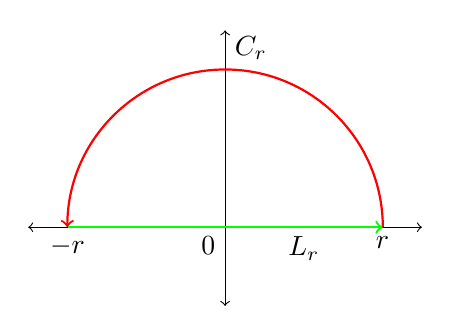
\begin{tikzpicture}

\draw[black, <->] (-2.5,0)--(2.5,0);
\draw[black, <->] (0,-1)--(0,2.5);

\draw[red, ->, thick] ([shift = (0:57pt)] 0,0) arc (0:180:57pt);

\draw[green, ->, thick] (-2,0) -- (2,0);


\draw (0,2) node[above right] {$C_{r}$};

\draw (1,0) node[below] {$L_r$};
\draw (0,0) node[below left] {$0$};
\draw (2,0) node[below] {$r$};
\draw (-2,0) node[below] {$-r$};
\end{tikzpicture}
\end{center}

If $f(z) = \frac{z+1}{z^4 + 2z^2 + 1}$, then the integral we care about is:

$$\int_{-\infty}^\infty f(x)dx = \lim_{r\rightarrow \infty} \int_{-r}^r f(x)dx = \lim_{r\rightarrow \infty} \int_{L_r}f(z)dz$$

To compute this, we'll proceed in three steps:

\begin{enumerate}
\item Show that $\lim_{r\rightarrow \infty} \int_{C_r} f(z)dz = 0$.
\item Show that $\int_{-\infty}^\infty f(z)dz = \lim_{r\rightarrow \infty} \int_{L_r + C_r} f(z)dz$.
\item Compute $\lim_{r\rightarrow \infty} \int_{L_r + C_r} f(z)dz$.
\end{enumerate}

\paragraph{Step 1.} To do this, we'll use M-L estimation (\ref{thm:mlest}). Since $C_r$ is a semicircle of radius $r$, it has length $L = \pi r$.

So we need to estimate the maximum of $|f(z)|$ on $C_r$. Since $f(z) = \frac{z+1}{z^4 + 2z^2 + 1}$, we can get an upper bound for $|f(z)|$ by getting an upper bound for $|z^2|$ and a lower bound for $|z^4 + 2z^2 + 1|$.

By the triangule inequality, $|z+1| \le |z| + 1$. Since $z$ is on $C_r$, $|z| = r$. So $|z+1| \le r+1$.

Also, by a variation of the triangle inequality (specifically that $|a-b| \ge ||a|-|b|$), we see that $|z^4+2z^2+1| \ge r^4 - 2z^2 - 1$ for $r$ large enough (bigger than 2 should be enough.)

Putting these two bounds together, we see that $|f(z)| \le \frac{r+1}{r^4 - 2r^2 - 1}$. And so, M-L esitmation gives us that:

$$\left| \int_{C_r} f(z)dz \right| \le \frac{\pi r(r+1)}{r^4 - 2r^2 -1}$$.

So, in the limit:

$$0 \le \lim_{r\rightarrow \infty} \left| \int_{C_r} f(z)dz \right| \le \lim_{r\rightarrow \infty}\frac{\pi r(r+1)}{r^4 - 2r^2 -1} = 0$$

And so $\lim_{r\rightarrow \infty} \int_{C_r} f(z)dz = 0$.

\paragraph{Step 2:} We know that:

$$\int_{-\infty}^\infty f(x)dx = \lim_{r\rightarrow \infty} \int_{L_r}f(z)dz$$

But since $ \lim_{r\rightarrow \infty} \int_{C_r}f(z)dz = 0$, we have that:

$$\int_{-\infty}^\infty f(x)dx = \lim_{r\rightarrow \infty} \int_{L_r}f(z)dz + \lim_{r\rightarrow \infty} \int_{C_r}f(z)dz =\lim_{r\rightarrow \infty} \int_{L_r+C_r}f(z)dz$$

\noin which is what we wanted to show.

\paragraph{Step 3:} We compute this integral using the residue theorem. Since $z^4+2z^2 + 1 = (z^2+1)^2$, we see that $f(z)$ has two double poles: $\pm i$. Of these, only $i$ is inside the curve (when $r > 1$). As such, when $r > 1$ the residue theorem gives:

$$\int_{L_r + C_R} f(z)dz = 2\pi i \Res\left(\frac{z+1}{z^4+2z^2 +1}; i\right)$$

Since this is a double pole, we compute:

\begin{align*}\Res\left(\frac{z+1}{z^4+2z^2 +1}; i\right) &= \lim_{z\rightarrow i} \frac{d}{d\,z} \frac{(z-i)^2(z+1)}{(z^2+1)^2}\\
&= \lim_{z\rightarrow i} \frac{d}{d\,z} \frac{z+1}{(z+i)^2}\\
&= \lim_{z\rightarrow i} \frac{(z+i)^2 -2(z+i)(z+i)}{(z+i)^4}\\
&=\frac{(2i)^2 - 2(2i)(i+1)}{(2i)^4}\\
&= \frac{-4 +4 -4i}{16}\\
&= \frac{-i}{4}
\end{align*}

And so, all together:

$$\int_{-\infty}^\infty f(x)dx = \lim_{r\rightarrow \infty} \int_{L_r+C_r}f(z)dz = 2\pi i\frac{-i}{4} = \frac{\pi}{2}$$

\end{ex}

For other rational functions, the procedure is identical.


\subsection{Contour Integration - Trig Functions}

We can also evaluate integrals that look like $\int_{-\infty}^\infty \frac{\cos(x)}{p(x)}dx$ and $\int_{-\infty}^\infty \frac{\sin(x)}{p(x)}dx$ as long as $\deg p(x) \ge 2$ and $p(x)\ne 0$ on $\R$.

The procedure to evaluate such an integral is very similar to working with rational functions. The only difference is that $\cos(z)$ and $\sin(z)$ aren't bounded on the upper half plane. So we need to get clever. The trick is to note that $\cos(z) = \RE(e^{iz})$ and $\sin(z) = \IM(e^{iz})$. We can then make use of the fact that $e^{iz}$ is bounded on the upper half plane.


\begin{ex}{}{} Find $\int_{-\infty}^\infty \frac{\sin(x)}{x^2+ 1}dx$.

Notice that $\left|\frac{\sin(x)}{x^2+1}\right| \le \frac{1}{x^2+1}$, so this integral converges absolutely by the basic comparison test. Absolutely convergent improper integrals converge, so this integral exists.

We're interested in $\int_{-r}^r \frac{\sin(x)}{x^2 +1}dx$. As in the previous example, we look at:

\begin{center}
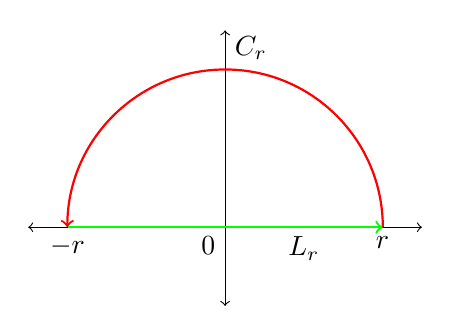
\begin{tikzpicture}

\draw[black, <->] (-2.5,0)--(2.5,0);
\draw[black, <->] (0,-1)--(0,2.5);

\draw[red, ->, thick] ([shift = (0:57pt)] 0,0) arc (0:180:57pt);

\draw[green, ->, thick] (-2,0) -- (2,0);


\draw (0,2) node[above right] {$C_{r}$};

\draw (1,0) node[below] {$L_r$};
\draw (0,0) node[below left] {$0$};
\draw (2,0) node[below] {$r$};
\draw (-2,0) node[below] {$-r$};
\end{tikzpicture}
\end{center}

Unlike in our previous example, $\sin(z)$ is not bounded on this curve. The trick here is to look at a slightly different integral: $\int_{-r}^r \frac{e^{ix}}{x^2+1}dx$. Notice that $\sin(x) = \IM(e^{ix})$ and so $\int_{-r}^r \frac{\sin(x)}{x^2+1}dx  = \IM \left(\int_{-r}^r \frac{e^{ix}}{x^2+1}dx\right)$.


Set $f(z) = \frac{e^{iz}}{z^2+1}$, so that the integral we care about is:

$$\int_{-\infty}^\infty f(x)dx = \lim_{r\rightarrow \infty} \int_{-r}^r f(x)dx = \lim_{r\rightarrow \infty} \int_{L_r}f(z)dz$$

To compute this, we'll proceed in three steps:

\begin{enumerate}
\item Show that $\lim_{r\rightarrow \infty} \int_{C_r} f(z)dz = 0$.
\item Show that $\int_{-\infty}^\infty f(z)dz = \lim_{r\rightarrow \infty} \int_{L_r + C_r} f(z)dz$.
\item Compute $\lim_{r\rightarrow \infty} \int_{L_r + C_r} f(z)dz$.
\end{enumerate}

\paragraph{Step 1.} To do this, we'll use M-L estimation (\ref{thm:mlest}). Since $C_r$ is a semicircle of radius $r$, it has length $L = \pi r$.

So we need to estimate the maximum of $|f(z)|$ on $C_r$. Since $f(z) = \frac{e^{iz}}{z^2 + 1}$, we can get an upper bound for $|f(z)|$ by getting an upper bound for $|e^{iz}|$ and a lower bound for $|z^2 +1|$.

Since $|e^{iz}| = e^{-\IM(z)} \le 1$ on $C_R$ and $|z^2+1| \ge R^2 - 1$ on $C_R$ for $R > 1$ by the triangle inequality, we see that $f(z) \le \frac{1}{R^2-1}$ on $C_R$ for $R>1$.

And so, M-L esitmation gives us that:

$$\left| \int_{C_r} f(z)dz \right| \le \frac{\pi r}{r^2 - 1}$$.

So, in the limit:

$$0 \le \lim_{r\rightarrow \infty} \left| \int_{C_r} f(z)dz \right| \le \lim_{r\rightarrow \infty}\frac{\pi r}{r^2  -1} = 0$$

And so $\lim_{r\rightarrow \infty} \int_{C_r} f(z)dz = 0$.

\paragraph{Step 2:} We know that:

$$\int_{-\infty}^\infty f(x)dx = \lim_{r\rightarrow \infty} \int_{L_r}f(z)dz$$

But since $ \lim_{r\rightarrow \infty} \int_{C_r}f(z)dz = 0$, we have that:

$$\int_{-\infty}^\infty f(x)dx = \lim_{r\rightarrow \infty} \int_{L_r}f(z)dz + \lim_{r\rightarrow \infty} \int_{C_r}f(z)dz =\lim_{r\rightarrow \infty} \int_{L_r+C_r}f(z)dz$$

\noin which is what we wanted to show.

\paragraph{Step 3:} We compute this integral using the residue theorem. Since $z^2+1 = (z-i)(z+i)$, we see that $f(z)$ has two simple poles: $\pm i$. Of these, only $i$ is inside the curve (when $r > 1$). As such, when $r > 1$ the residue theorem gives:

$$\int_{L_r + C_R} f(z)dz = 2\pi i \Res\left(\frac{e^{iz}}{z^2 +1}; i\right)$$

Since this is a simple pole, we compute:

\begin{align*}\Res\left(\frac{e^{iz}}{z^2+1}; i\right) &= \lim_{z\rightarrow i} \frac{(z-i)e^{iz}}{z^2+1}\\
&= \lim_{z\rightarrow i} \frac{e^{iz}}{z+i}\\
&= \frac{e^{-1}}{2i}
\end{align*}

And so, all together:

$$\int_{-\infty}^\infty f(x)dx = \lim_{r\rightarrow \infty} \int_{L_r+C_r}f(z)dz = 2\pi i\frac{1}{2ei} = \frac{\pi}{e}.$$

So, we have that $\int_{-\infty}^\infty \frac{\sin(x)}{x^2+1}dx = \IM \left(\int_{-\infty}^\infty f(x)dx\right) = \IM\left(\frac{\pi}{e}\right) = 0$.

\end{ex}